%%%%%%%%%%%%%%%%%%%%%%%%%%%%%%%%%%%%%%%%%
% Manuel d'utilisation du projet Picross de l'équipe Craketeam
% 
%%%%%%%%%%%%%%%%%%%%%%%%%%%%%%%%%%%%%%%%%

%----------------------------------------------------------------------------------------
%	Packages et documention du document
%----------------------------------------------------------------------------------------

\documentclass[11pt]{article}

\usepackage{fancyhdr} % Required for custom headers
\usepackage{lastpage} % Required to determine the last page for the footer
\usepackage{extramarks} % Required for headers and footers
\usepackage[usenames,dvipsnames]{color} % Required for custom colors
\usepackage{graphicx} % Required to insert images
\usepackage{listings} % Required for insertion of code
\usepackage{courier} % Required for the courier font
\usepackage[utf8]{inputenc}
\usepackage{indentfirst} %Indentation début de paragraphe
\usepackage{float}
\usepackage{colortbl} %Clouleur tableau protoypes de fonctions
\usepackage{tabularx}
\usepackage{placeins}


% Marges
\topmargin=-0.45in
\evensidemargin=0in
\oddsidemargin=0in
\textwidth=6.5in
\textheight=9.0in
\headsep=0.25in

\linespread{1.1} % Line spacing

% Réglages des pieds de page et des en-têtes
\pagestyle{fancy}
\lhead{\hmwkAuthorName} % Top left header
\chead{\hmwkClass\ - \hmwkTitle} % Top center head
\rhead{\firstxmark} % Top right header
\lfoot{\lastxmark} % Bottom left footer
\cfoot{} % Bottom center footer
\rfoot{Page\ \thepage\ sur\ \protect\pageref{LastPage}} % Bottom right footer
\renewcommand\headrulewidth{0.4pt} % Size of the header rule
\renewcommand\footrulewidth{0.4pt} % Size of the footer rule

\setlength\parindent{10pt} % Removes all indentation from paragraphs


\newcommand{\hmwkTitle}{PROJET JEU} % Titre du document
\newcommand{\hmwkDueDate}{Mercredi 14 mai 2014} % Date
\newcommand{\hmwkClass}{MANUEL D'UTILISATION } % Type de document
\newcommand{\hmwkClassInstructor}{ } % Teacher/lecturer
\newcommand{\hmwkAuthorName}{Groupe A} % Your name
\newcommand{\hmwkAuthorClasse}{L3 info SPI} % Classe


%----------------------------------------------------------------------------------------
%	Page de Titre
%----------------------------------------------------------------------------------------

\title{
\pagenumbering{roman} \setcounter{page}{0} %La page courante sera numérotée en roman et aura l'indice 0 => Pas de numéro car pas de 0 en roman
\vspace{2in}
\textmd{\textbf{\hmwkClass:\ \hmwkTitle}}\\
\normalsize\vspace{0.1in}\small{\hmwkDueDate}\\
\vspace{0.1in}\large{\textit{\hmwkClassInstructor\ }}
\vspace{3in}
}

\author{\textbf{\hmwkAuthorName}}


\date{\hmwkAuthorClasse} % Insert date here if you want it to appear below your name

%----------------------------------------------------------------------------------------

\begin{document}

\thispagestyle{empty}
\maketitle
\newpage


%----------------------------------------------------------------------------------------
%	Table de matières
%----------------------------------------------------------------------------------------

\thispagestyle{empty}
\pagenumbering{arabic} \setcounter{page}{0} %Le reste du document est numéroté en arabic à partir de la page 1
\renewcommand\contentsname{Sommaire}
\tableofcontents
\newpage


%----------------------------------------------------------------------------------------
%	Présentation générale
%----------------------------------------------------------------------------------------

\newpage

\section{Description du manuel}

\subsection{Contexte}

Ce manuel d’utilisation est créé dans le cadre d’un projet étudiant durant le 2ème semestres de L3 SPI informatique. Il concentre toutes les informations essentielles à l’utilisateur lors des premières utilisations. 

\subsection{Objectif}

L’objectif de ce manuel est de guider l’utilisateur sur l'application picross lors des premières utilisations, il doit aussi pouvoir expliquer des différentes fonctionnalitées de l'application. 

\section{Démarrage}

\subsection{Prérequis}

Pour pouvoir lancer l'application picross la machine doit avoir ruby et ses dépendances aux préalable.

Si ce n'est pas le cas veuillez vivre les différentes précédures en fonction de votre Système d'exploitation :

	\begin{itemize}
		\item Mac : http://hop3x.univ-lemans.fr/MacOsX-RubyGtk.html
		\item Linux : http://hop3x.univ-lemans.fr/Linux-RubyGtk.html
		\item Windows : http://hop3x.univ-lemans.fr/Windows-RubyGtk.html
	\end{itemize}

\subsection{Lancer l'application}

Une fois ruby installé sur votre machine : 
	
	\begin{itemize}
		\item Ouvrez un terminal
		\item Placez vous dans le dossier dans lequel vous avez mis le dossier de l'application
		\item Puis taper la ligne de commande suivante : "ruby NouveauxJeu.rb"
	\end{itemize}

%----------------------------------------------------------------------------------------
%	Manuel
%----------------------------------------------------------------------------------------

\newpage


\section{Manuel Utilisateur}


\subsection{Accueil Visiteur}

L'accueil visiteur est la fenêtre qui s'affiche lors du lancement de l'application. C'est une fenêtre qui permet d'accèder aux différentes fonctionnalitées de l'application à travers de bouton.

Elle permet l'accès à :

	\begin{itemize}
		\item Une partie rapide
		\item La création ou le chargement d'un profil
		\item Les options
		\item Les crédits
	\end{itemize}

Il est bien sûr possible de quitter l'application à travers le bouton "quitter" et à tout moment grâce à la croix en haut à droite.

	\begin{figure}[!h]
		\centering
		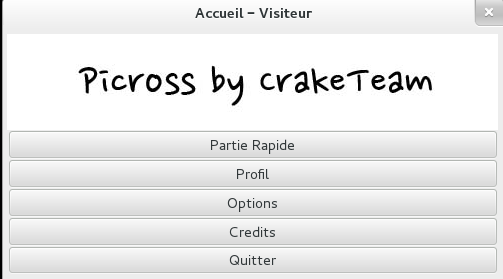
\includegraphics[width=10cm]{./Screenshot/AccueilVisiteur.png}
		\caption{Fenêtre d'Accueil Visiteur}
	\end{figure}

Pour plus d'information veuillez consulter les rubriques respective des éléments cités ci-dessus dans la suite de ce document.

\newpage

\subsection{Le Profil}

	\begin{figure}[!ht]
		\centering
		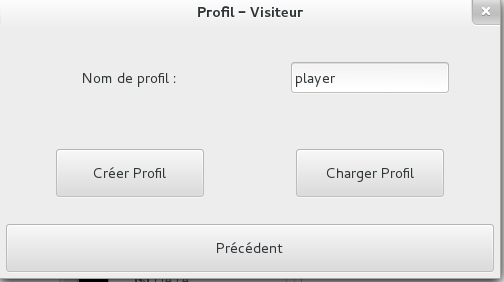
\includegraphics[width=10cm]{./Screenshot/Profil.png}
		\caption{Fenêtre de création et de chargement de Profil}
	\end{figure}

Sur cette fenêtre en rentrant un pseudo dans le champs texte on peut soit le créer soit le charger s'il est déjà existant grâce aux deux bouton "Créer profil" et "Charger Profil"

Le bouton Précédent permet de revenir à l'Accueil Visiteur.	

\subsection{Options}

Ici nous pouvons changer les différentes options que propose l'application du picross.

	\begin{figure}[!ht]
		\centering
		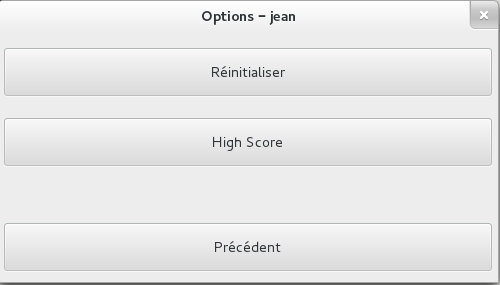
\includegraphics[width=10cm]{./Screenshot/Options.png}
		\caption{Fenêtre des Options}
	\end{figure}

\newpage

\subsection{Credits}

Page listant les différents membre et de leur poste dans l'équipe du projet CrakeTeam.

	\begin{figure}[!ht]
		\centering
		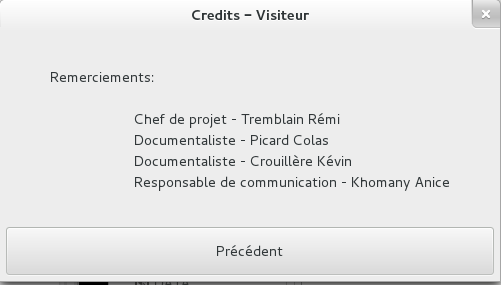
\includegraphics[width=10cm]{./Screenshot/Credits.png}
		\caption{Fenêtre des Crédits}
	\end{figure}


\subsection{Paramètre d'une partie}

Lorsque l'on veut lancer une nouvelle partie, il faut précisé ses différents paramètres telle que la taille de la grille et la difficulté de l'aide (voir ci-dessous)

	\begin{figure}[!ht]
		\centering
		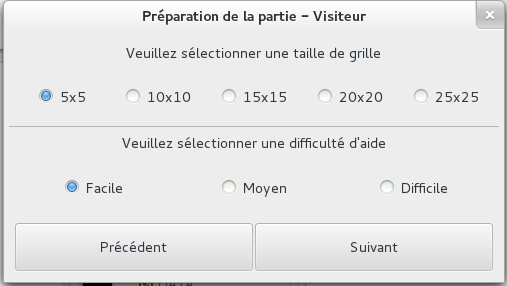
\includegraphics[width=10cm]{./Screenshot/PrepaPartie.png}
		\caption{Fenêtre de Préparation de la partie}
	\end{figure}


Une fois cela fait un choix de la grille est disponible offrant plusieur possibilité :
	
	\begin{itemize}
		\item La Grille aléatoire - génére une grille aléatoirement
		\item Toutes les grilles - choix d'une grille parmis toutes les grilles qu'on créer tout les utilisateurs dans l'édition de grille
		\item Grille perso - permet de charger une grille enregistrer (Option uniquement disponible lorsque l'on est connecter à un profil)
	\end{itemize}

	\begin{figure}[!ht]
		\centering
		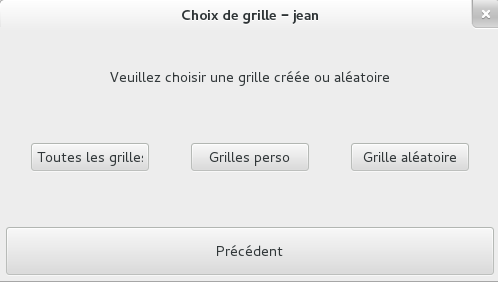
\includegraphics[width=10cm]{./Screenshot/ChoixGrille.png}
		\caption{Fenêtre de choix de grille}
	\end{figure}

\newpage

\subsection{Accueil Profil}

La nouveauté de cette Accueil est l'accés à l'Editeur de grille à traver le bouton "Editeur", Ah par celà elle propose principalement les mêmes possibilités que l'accueil visiteur (voir plus haut sur ce document).

	\begin{figure}[!ht]
		\centering
		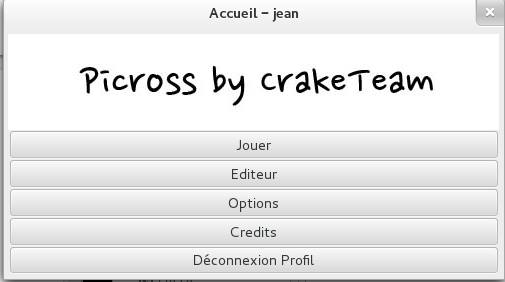
\includegraphics[width=10cm]{./Screenshot/AccueilProfil.png}
		\caption{Fenêtre Accueil Profil}
	\end{figure}

\newpage

\subsection{Editeur}

Après avoir choisis une taille de grille, Il suffit de cliquer aux endroit où l'on veut que les cases soit noircie dans la grille et de cliquer sur Enregistrer.

	\begin{figure}[!ht]
		\centering
		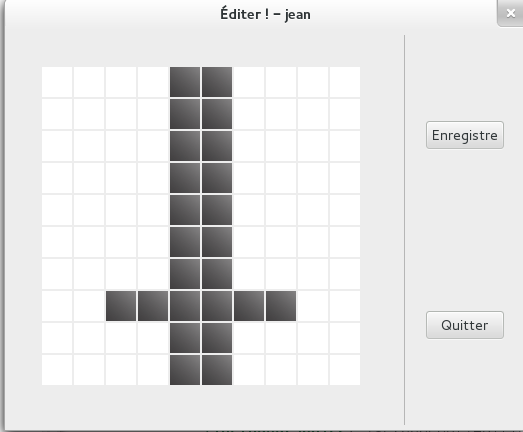
\includegraphics[width=10cm]{./Screenshot/Editeur.png}
		\caption{Fenêtre d'Edition de grille}
	\end{figure}

\end{document}
